\section{Reference value}

Our benchmarking framework will compute the context switching time but we need to know how well or how bad our framework performs.
To assess the performance of our measurements, we first need to compute the real context switching time.
This real context switching time will be our reference value.

\subsection{Simple task}
In order to experiment and test our benchmarking framework, we need to have a simple application on every tested RTOS.

The application contains two indentical tasks.
The tasks wait for 1ms in the foreground and then goes to the background letting the scheduler runs the next task.
The tasks run in an infinite loop.

\subsubsection{Implementation in Contiki}
The source code of one of the two tasks is shown in the listing \ref{lst:simple-task-code}.
It uses the \texttt{clock\_delay\_usec()} call to make the task wait for 1ms.
Finally, we use the \texttt{PROCESS\_PAUSE()} macro to pause the task and let the other task do its iteration.

\begin{lstlisting}[style=CStyle, float, label={lst:simple-task-code}, caption={Source code of a task implemented in Contiki for the simple application}]
PROCESS_THREAD(task, ev, data)
{
    PROCESS_BEGIN();

    while (1)
    {
        clock_delay_usec(1000);
        PROCESS_PAUSE();
    }

    PROCESS_END();
}
\end{lstlisting}

\subsubsection{Implementation in RIOT OS}
The source code of on of the two tasks is shown in the listing \ref{lst:simple-task-code-riot}.
We can not use the \texttt{xtimer\_usleep()} method as it will lead to a context switch.
Instead, we used a for loop.
The \texttt{thread\_yield()} call will perfom a context switch and let the other task run on iteration.

\begin{lstlisting}[style=CStyle, float, label={lst:simple-task-code-riot}, caption={Source code of a task implemented in RIOT OS for the simple application}]
void *threadA(void *arg)
{
    (void)arg;

    while (1)
    {
        for(int i = 0; i < 1000; i++) {}
        thread_yield();
    }
    return NULL;
}
\end{lstlisting}


\subsection{Methodology}

In order to compute the real context switching time, we used an oscilloscope and two GPIOs.
Each task of our simple application is responsible of one GPIO.
Every time a task is run and goes to the foreground, it sets its GPIO up.
Once the task is finished and goes to the background, it resets its GPIO down.

With the oscilloscope, we can mesure the voltage of the two GPIOs and compute the real context switching time from those measurements.
The figure \ref{fig:real-context-switching-time-measurement} shows the different steps of our methodology.
On this schema, the execution time of the two tasks are represented above the voltage measurements of the two GPIOs.
The context switching time happens between the execution of the two tasks and is bordered with dotted lines.

\begin{figure}[!ht]
  \centering
  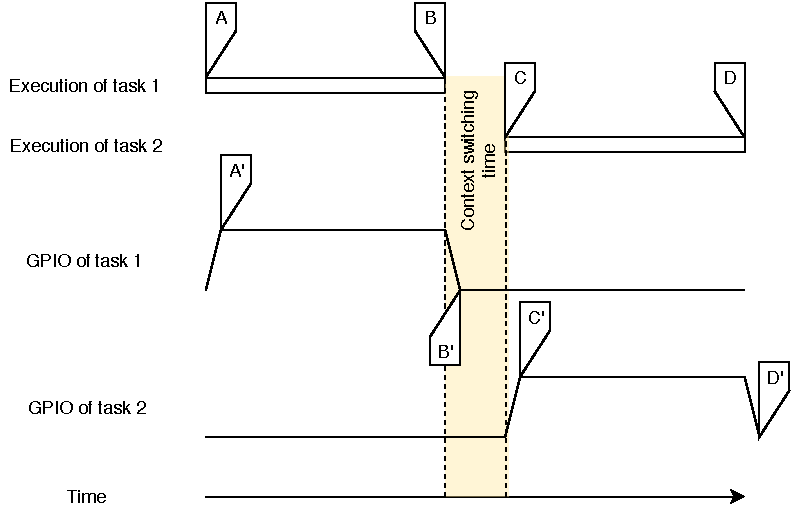
\includegraphics[scale=1]{assets/real-context-switching-time-measurement.pdf}
  \caption{\label{fig:real-context-switching-time-measurement}Steps in the methodology to compute the real context switching time}
\end{figure}

The steps are the following.
The first task sets up its GPIO on step A.
The GPIO is in high position few nano seconds later on step A'.
Once the first task is over, it resets its GPIO on step B which goes in low position on step B'.
In the same way, the second task set up its GPIO on step C which goes in high position on step C' few nano seconds later and reset it on step D which goes in low position on step D'.
The oscilloscope measures the context switching time between the step B' and the step C'.
The time for the GPIOs to rise up or down are around 10 nano seconds and can be omitted.


\subsection{Measurement setup}

The oscilloscope used for the measurement was the \href{https://www.tek.com/oscilloscope/mso56}{Tektronix MSO 56} available at the Welcome Lab at UCLouvain.
We used two channels to measure the voltage of the two GPIOs used by the application.

We updated our simple task by adding GPIO calls in order for the oscilloscope to detect it.
The task will set up a GPIO, wait for 1ms, and then clear the GPIO.
The two tasks use different GPIO in order to differenciate them with the oscilloscope.

\subsubsection{Implementation in Contiki}
The source code of the updated task is shown in the listing \ref{lst:gpio-task-code}.
\texttt{GPIO\_SET\_PIN()} and \texttt{GPIO\_CLR\_PIN()} are used to respectively set and clear the GPIO used by the task.

\begin{lstlisting}[style=CStyle, float, label={lst:gpio-task-code}, caption={Source code of the task with GPIO calls}]
  PROCESS_THREAD(task, ev, data)
  {
      PROCESS_BEGIN();
  
      while (1)
      {
          GPIO_SET_PIN(
              GPIO_PORT_TO_BASE(GPIO_C_NUM), 
              GPIO_PIN_MASK(3));

          clock_delay_usec(1000);

          GPIO_CLR_PIN(
              GPIO_PORT_TO_BASE(GPIO_C_NUM), 
              GPIO_PIN_MASK(3));

          PROCESS_PAUSE();
      }
  
      PROCESS_END();
  }
\end{lstlisting}

\subsubsection{Implemetation in RIOT OS}
The source code of the updated task is shown in the listing \ref{lst:gpio-task-code-riot}.
\texttt{gpio\_set()} and \texttt{gpio\_clear()} are used to respectively set and clear the GPIO used by the task.

\begin{lstlisting}[style=CStyle, float, label={lst:gpio-task-code-riot}, caption={Source code of a task implemented in RIOT OS for the simple application}]
    void *thread(void *arg)
    {
        (void)arg;
    
        while (1)
        {
            gpio_set(GPIO_PIN(PORT_C, 2));

            for(int i = 0; i < 1000; i++) {}

            gpio_clear(GPIO_PIN(PORT_C, 2));

            thread_yield();
        }
        return NULL;
    }
    \end{lstlisting}

\subsection{Measurement results}

% The figure \ref{fig:measurement-value-wave} shows concretely the measurements made by our oscilloscope.
% As described in the methodology, high values means that the task is running in the foreground and low values means that the task is sleeping in the background.

% \begin{figure}[!ht]
%   \centering
%   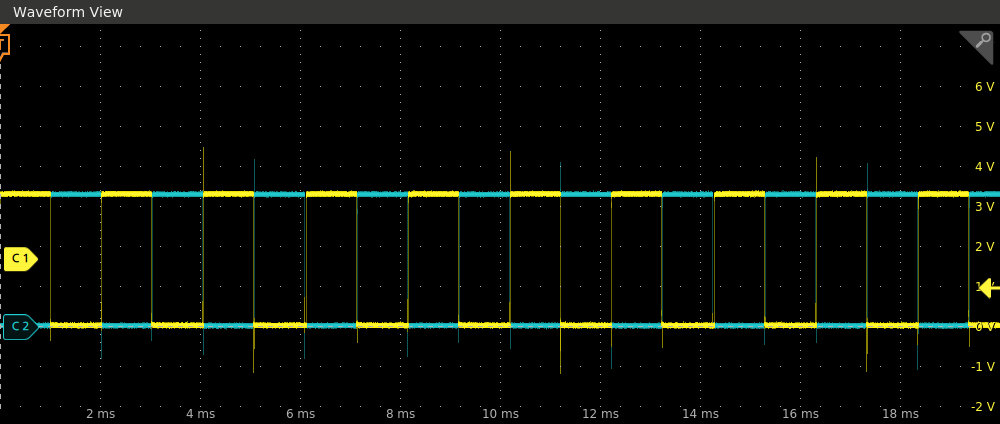
\includegraphics[scale=0.5]{assets/measurement-value-wave.png}
%   \caption{\label{fig:measurement-value-wave}Voltage measurement of the two GPIOs; Each color represents a task}
% \end{figure}

% The context switching time is the time during which no task is running.
% This is visible with the oscilloscope when both channels are low.

% With the oscilloscope, we made four measurements.
% The first two measurements are the context switching times from task 1 to task 2 and from task 2 to task 1.
% The other two measurements are the time taken by the two tasks.
% These last measurements should be arround 1ms.
% The measurements are shown in the table \ref{tab:reference-measurement}.

% With these results, we can see that the duration of both tasks is 1ms with no variation.
% We also extract with this measurement our reference value.
% From task 1 to task 2, we have 14.68$\mu$s of context switching time and from task 2 to task 1, we have 14.88$\mu$s.
% Our benchmarking framework should compute the context switching time of that same application and output a value between 13.30$\mu$s and 16.26$\mu$s.

% \begin{table}[!ht]
%   \centering
%   \begin{tabular}{llll}
%                         & \multicolumn{3}{c}{Time ($\mu$s)}                              \\ \cline{2-4} 
%                         & \multicolumn{1}{c}{Mean} & Min   & \multicolumn{1}{c}{Max} \\ \cline{2-4} 
%   From task 1 to task 2 & 14.68                    & 14.35 & 14.79                   \\
%   From task 2 to task 1 & 14.88                    & 14.33 & 14.97                   \\
%   Duration of task 1    & 1003                     & 1003  & 1003                    \\
%   Duration of task 2    & 1003                     & 1003  & 1003                   
%   \end{tabular}
%   \caption{Context switching times and task durations measured with the oscilloscope Tektronix MSO 56}
%   \label{tab:reference-measurement}
% \end{table}